%\documentclass[../main.tex]{subfiles}


\begin{song}{title=\centering Do dne a do roka \\ \normalsize Jaromír Nohavica \vspace*{-0.3cm}}  %% sem se napíše jméno songu a autor
%\fontsize{10pt}{12pt}\selectfont
\begin{minipage}{0.60\textwidth}
\moveright 3.8cm \vbox{      %Varianta č. 1  ---> Jeden sloupec zarovnaný na střed
\setcounter{Slokočet}{0}

\sloka
Byla ^{Hmi}hluboká noc, ^{C#mi7}venku ^{F#mi}cizí pes vyl 

a ja ^{Hmi}u okna stál ^{C#mi7}a ^{F#mi}pil. 

Zřel jsem jen ^{Hmi}jeho stín, ^{C#mi7}měl ^{F#mi}rozplizlý tvar 

a ^{Hmi}vypadal jak ^{C#mi7}Lomi^{F#mi}kar 


\refren
Do dne a ^{Hmi}do roka, za zvuku ^{C#mi7}baroka, se rodí ^{F#mi}rokoko.

Do noci ^{Hmi}hledíme, a vlastně ^{C#mi7}nevíme, 

zda je to ^{F#mi}opravdu anebo jenom tak, naoko. 

Do dne a ^{Hmi}do roka, za zvuku ^{C#mi7}rokoka, se rodí ^{F#mi}secese. 

Do noci ^{Hmi}hledíme, všichni tam ^{C#mi7}musíme, ale ^{F#mi}nechce se. 

\sloka
Chtěl jsem okřiknout jej, myslím psa v oné tmě, 

ale neměl jsem slov, jimiž to lze.

Vzal jsem do ruky kolt, jenž v mé komodě byl 

a na černý stín jsem namířil. 

\refren

\sloka
Ruka chvěla se mi, neboť z krbu šel mráz,

pak se na vteřinu zastavil čas. 

Tmě se zježila srst, já ucítil strach, 

kdo má na spoušti prst, je vrah.

\refren

\sloka
Výstřel protrhl tmu jako rybářům síť,

jako sudičce řeč a niť. 

Té noci špatně jsem spal v záři voskových svic,

ráno tam, co byl plot, nebylo nic. 

\refren

}
\end{minipage}
\begin{minipage}{0.38\textwidth}
\moveright .5cm \vbox{
	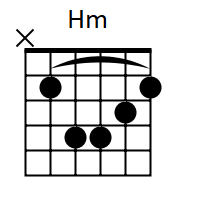
\includegraphics[width=2.5cm]{../Akordy/hm.png}
	
	
\includegraphics[width=2.5cm]{../Akordy/cxm7.png}
	
	
\includegraphics[width=2.5cm]{../Akordy/fxm.png}
}
\end{minipage}
\end{song}



%\begin{figure}[h]
%	\centering
%	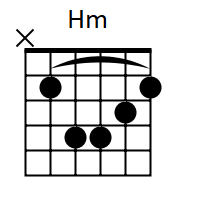
\includegraphics[scale=0.8]{../Akordy/hm}
%	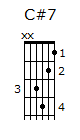
\includegraphics[scale=1.5]{../Akordy/cx7}
%	\includegraphics[scale=1.5]{../Akordy/fxm7
%\end{figure}
